%-------------------------------------------------------------------------------
%	PAQUETES Y OTRAS CONFIGURACIONES
%-------------------------------------------------------------------------------

%----------------------------------------------------------------------------------------
%	PAQUETES Y OTRAS CONFIGURACIONES
%----------------------------------------------------------------------------------------

%\documentclass[paper=letter, fontsize=11pt]{scrartcl} % Tamaño de papel y letra para el documento
\documentclass{tufte-handout}

\usepackage[utf8]{inputenc} % Los caracteres acentuados se pueden escribir normalmente en el código
\usepackage[T1]{fontenc} % Configuración de fuente de salida
\usepackage{fourier} % Se usa una fuente diferente al default
\usepackage[spanish,es-noquoting]{babel} % Se configura como documento en español
\usepackage{amsmath,amsfonts,amsthm} % Paquetes para escribir formulas matemáticas
\usepackage{graphicx} % Paquetes para incluir imágenes

\usepackage{circuitikz}
\usepackage{tikz}
\usetikzlibrary{arrows}

\usepackage{sectsty} % Paquete para configuración de secciones
\allsectionsfont{\centering \normalfont \scshape} % Los títulos de las secciones son centrados, con la misma fuente y pequeñas mayúsculas

\usepackage{todonotes}
\usepackage{microtype}

\usepackage{fancyhdr} % Paquete para personalizar pies y cabeceras de página
\pagestyle{fancyplain} % Todas las páginas con las mismas cabeceras y pies de página
\fancyhead{} % Sin cabecera
\fancyfoot[L]{} % Vacío en la izquierda del pie de página
\fancyfoot[C]{} % Vacío en el centro del pie de página
\fancyfoot[R]{\thepage} % Número de página en el pie de pagina
\renewcommand{\headrulewidth}{0pt} % Sin lineas en la cabecera
\renewcommand{\footrulewidth}{0pt} % Sin lineas en el pie de página
\setlength{\headheight}{13.6pt} % Altura de cabecera

\numberwithin{equation}{section} % Numera ecuaciones en cada sección
\numberwithin{figure}{section} % Numera figuras en cada sección
\numberwithin{table}{section} % Numera tablas en cada sección

\setlength\parindent{0pt} % Quita la indentación de los párrafos

\newcommand{\horrule}[1]{\rule{\linewidth}{#1}} % Comando personalizado para hacer linea horizontal


%-------------------------------------------------------------------------------
%	TITULO
%-------------------------------------------------------------------------------

\title{ Tarea 1 - Dinámica del robot }

\author{Roberto Cadena Vega} % Nombre del profesor

\date{ } % Fecha de la práctica

%-------------------------------------------------------------------------------
%	EMPIEZA EL DOCUMENTO
%-------------------------------------------------------------------------------

\begin{document}

\maketitle % Imprime el título
\begin{marginfigure}
	
\includegraphics[width=0.8\textwidth]{../images/UNITEC.png}
\end{marginfigure}
%-------------------------------------------------------------------------------
%	PROBLEMAS
%-------------------------------------------------------------------------------

\section{Problemas}

\begin{enumerate}

	\item El movimiento de una particula esta definido por la relación $x = 1.5t^4 - 30t^2 + 5t + 10$, en donde $x$ y $t$ son expresadas en metros y segundos respectivamente. Determine la posición, velocidad y aceleración de la particula en el tiempo $t = 4s$.

	\item El movimiento de una particula esta definido por la relación $x = 6t^2 - 8 + 40\cos{\pi t}$ en donde $x$ y $t$ estan expresadas en metros y segundos respectivamente. Determine la posición, velocidad y aceleración de la particula cuando $t = 6s$.

	\item Una bola de boliche es tirada desde un bote, de tal manera que la velocidad con la que entra al agua es de $25 \frac{ft}{s}$. Suponiendo que la bola experimenta una aceleración de $a = 10 - 0.9v^2$ mientras esta sumergida, determine la velocidad de la bola cuando llega al fondo del lago a $30 ft$ de la superficie.

	\item Un conductor entra a una autopista con una velocidad de $45 \frac{km}{h}$, y acelera uniformemente hasta que el velocimetro de su automovil marca $99 \frac{km}{h}$ y el odómetro marca una diferencia de $0.2 km$. Determine (a) la aceleración del automovil y (b) el tiempo requerido para llegar a la velocidad final de $120 \frac{km}{h}$ si continua con la misma aceleración.

	\item Un grupo de estudiantes lanza un cohete a escala en dirección vertical. Basados en los datos del acelerometro a bordo determinan que la altitud alcanzada en la parte propulsada del trayecto fue de $89.6ft$ y que aterrizó $16s$ despues de que se agotara su combustible. Sabiendo que el paracaidas de descenso falló y que el cohete cayo libremente al suelo, determine (a) La velocidad $v_1$ al final de la parte propulsada del trayecto y (b) la máxima altitud alcanzada por el cohete.

	\item Se descarga arena a traves de una banda transportadora hacia un monticulo a una distancia de $30 ft$ del extremo de la banda. Si los granos de arena impactan el monticulo $18 ft$ por debajo del extremo de la banda y la banda tiene una inclinación de $\alpha = 20^o$ con respecto a la horizontal, determine la velocidad $v_0$ de la banda.

	\begin{marginfigure}
		\begin{center}
			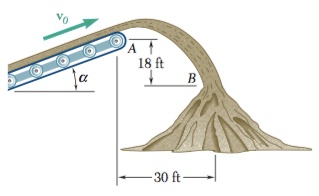
\includegraphics[width=\textwidth]{./images/arena.png}
		\end{center}
	\end{marginfigure}

	\newpage

	\item La velocidad inicial $v_0$ de un puck de hockey es de $105 \frac{mi}{h}$, determine (a) el mayor valor (menor a 45º) del angulo $\alpha$ para el cual el puck entrará en la red y (b) el tiempo que le tomará al puck alcanzar la red.

	\begin{figure*}
		\begin{center}
			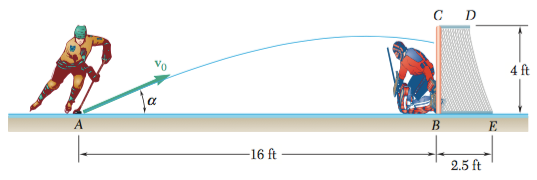
\includegraphics[width=0.6\textwidth]{./images/puck.png}
		\end{center}
	\end{figure*}

	\item Determine la velocidad máxima de un carro en una montaña rusa, de tal manera que en una curva con radio $\rho = 80ft$ la aceleración no sobrepase $3g$.

	\begin{marginfigure}
		\begin{center}
			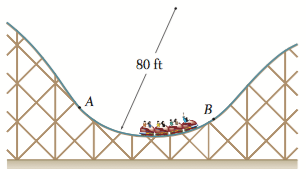
\includegraphics[width=\textwidth]{./images/rusa.png}
		\end{center}
	\end{marginfigure}

	\item Un automovilista que viaja a lo largo de una porción de la autopista, decrementa su velocidad hasta llegar a una salida con forma circular, con un radio de $560ft$, y continua desacelerando por $10s$ hasta tener una velocidad de $20 mi/h$ y mantenerla. Sabiendo que la aceleración que experimenta el automóvil en este trayecto es un cuarto de la aceleración antes de entrar a la rampa. Determine el maximo valor de aceleración total experimentada por el automóvil.

	\begin{marginfigure}
			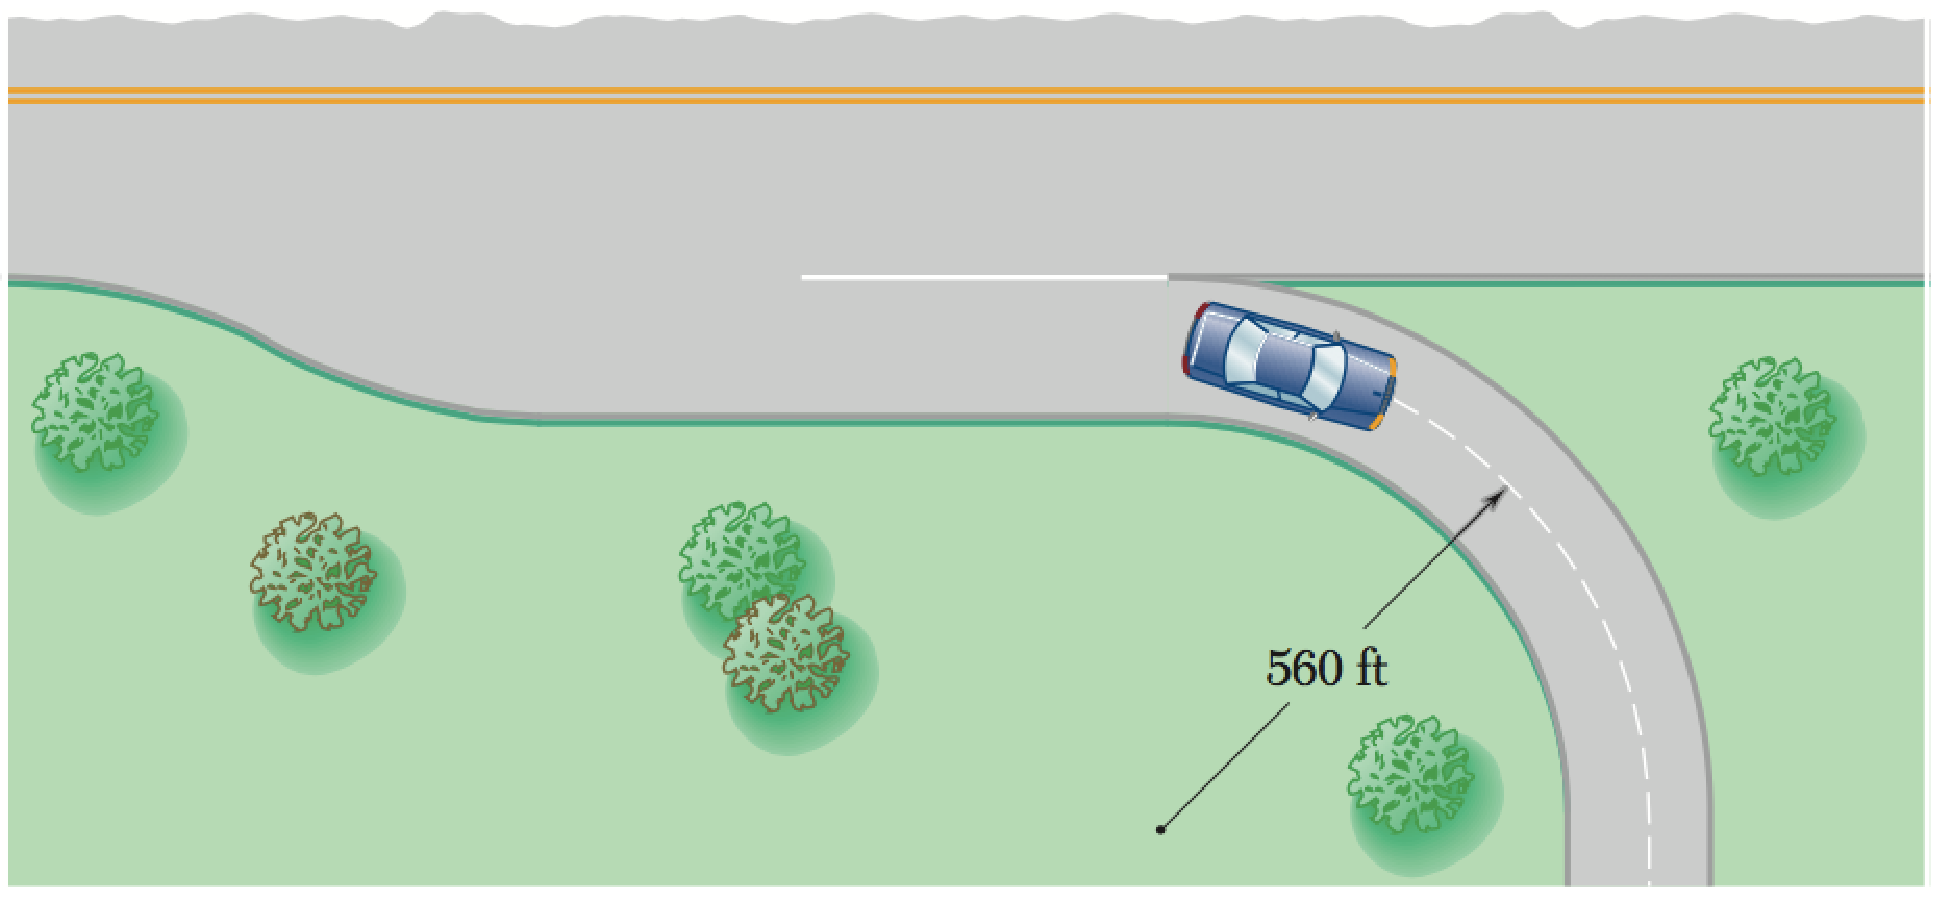
\includegraphics[width=\textwidth]{./images/auto.pdf}
	\end{marginfigure}

	\item Determine la velocidad de orbita del telescopio espacial Hubble, sabiendo que el radio de la tierra es $R = 6370km$, que el telescopio en cuestion, viaja en una orbita a $590km$ de la superficie de la tierra y que la aceleración debido a la gravedad en ese punto está determinada por la formula $g \left(\frac{R}{\rho} \right)^2$, en donde $\rho$ es el radio de la orbita.

\end{enumerate}

%-------------------------------------------------------------------------------
%	PROBLEMAS EXTRA
%-------------------------------------------------------------------------------

\section{Problemas extra}

\begin{enumerate}
	\item La aceleración de una particula esta definida por $a = -8 \frac{m}{s^2}$. Sabiendo que la posición de la particula es $x = 20m$ cuando $t = 4s$ y que la posición es $x = 4m$ cuando la velocidad es $v = 16 \frac{m}{s}$ determine (a) el tiempo $t_1$ cuando la velocidad es $0$, (b) la velocidad y distancia total recorrida cuando $t = 11s$.

	\item Determine el radio mínimo que debe ser usado en una salida de autopista si la componente normal de aceleración de un automovial viajando a $45 \frac{mi}{h}$ no debe exceder $2.4 \frac{ft}{s^2}.$

	\begin{marginfigure}
		\begin{center}
			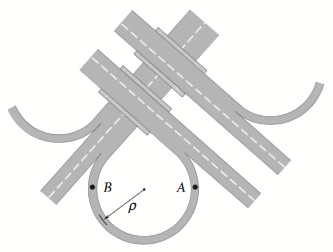
\includegraphics[width=\textwidth]{./images/autopista.png}
		\end{center}
	\end{marginfigure}
\end{enumerate}

%-------------------------------------------------------------------------------
%	FIN DEL DOCUMENTO
%-------------------------------------------------------------------------------

\end{document}
